\documentclass[aspectratio=169]{beamer}

% Theme selection
\usetheme{Madrid}
\usecolortheme{dove} % Light gray professional aesthetic

% Logo placement in top right
\addtobeamertemplate{frametitle}{}{%
\begin{tikzpicture}[remember picture,overlay]
\node[anchor=north east,yshift=-2pt] at (current page.north east) {
\includegraphics[height=0.8cm]{assets/logo.png}};
\end{tikzpicture}}

% Packages
\usepackage[utf8]{inputenc}
\usepackage[T1]{fontenc}
\usepackage{graphicx}
\usepackage{amsmath}
\usepackage{listings}
\usepackage{hyperref}
\usepackage{tikz}

% Metadata
\title[Transport Protocol Benchmarking]{Hardening a Network Benchmarking Laboratory}
\subtitle{Comparative Analysis of TCP and QUIC Congestion Control}
\author{Eyobed}
\institute{BUT PDSe}
\date{April 2026}

\begin{document}

% Title Slide
\begin{frame}
    \titlepage
\end{frame}

% Section 1: Objective
\section{Experimental Objective}
\begin{frame}{Experimental Objective}
    \begin{itemize}
        \item \textbf{Goal:} Evaluate transport protocol efficiency (TCP vs QUIC) in hostile network conditions.
        \item \textbf{Isolation:} Use Linux Network Namespaces to simulate isolated nodes.
        \item \textbf{Rigor:} Moving bottlenecks to the router egress to eliminate measurement artifacts.
        \item \textbf{Telemetry:} High-fidelity 50Hz polling of the Congestion Window (CWND).
    \end{itemize}
\end{frame}

% Section 2: Methodology
\section{Methodology & Topology}
\begin{frame}{Hardened Lab Topology}
    \begin{center}
        \includegraphics[width=0.7\textwidth]{assets/topology_diagram.png} % Placeholder for diagram
    \end{center}
    \begin{itemize}
        \item \textbf{Bottlenecking:} Forced 100Mbps TBF on Router \texttt{r\_out}.
        \item \textbf{Cleaning:} Mandatory \texttt{tc qdisc del} and offload disabling (TSO/GSO) before every run.
        \item \textbf{Isolation:} 40-second tests with localized servers to avoid `TIME_WAIT` pollution.
    \end{itemize}
\end{frame}

% Section 3: WiFi Scenario
\section{Scenario 1: Coffee Shop Wi-Fi}
\begin{frame}{Scenario 1: Coffee Shop Wi-Fi (3\% Loss)}
    \begin{columns}
        \begin{column}{0.5\textwidth}
            \begin{itemize}
                \item \textbf{Condition:} 100Mbps cap + 3\% random packet loss.
                \item \textbf{Reno/CUBIC:} Severe collapse due to false congestion identification.
                \item \textbf{BBR:} Immunity to random loss; maintains model-based throughput.
            \end{itemize}
        \end{column}
        \begin{column}{0.5\textwidth}
            \begin{center}
                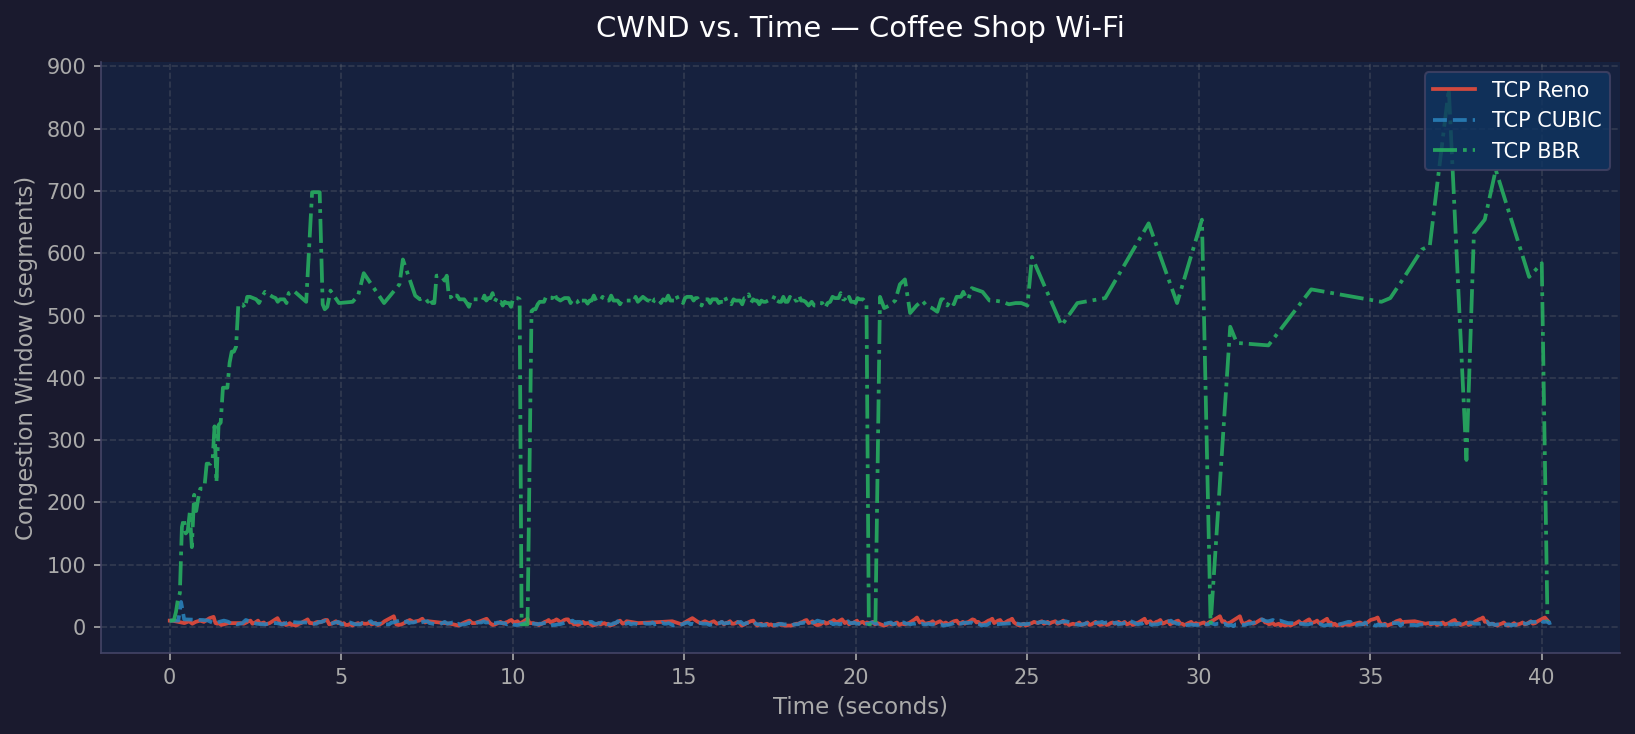
\includegraphics[width=\textwidth]{assets/plots/tcp_coffeeshop_wifi_cwnd.png}
            \end{center}
        \end{column}
    \end{columns}
\end{frame}

% Section 4: Satellite Scenario
\section{Scenario 2: Starlink Satellite}
\begin{frame}{Scenario 2: Starlink Satellite (600ms RTT + Jitter)}
    \begin{columns}
        \begin{column}{0.45\textwidth}
            \begin{itemize}
                \item \textbf{Observation:} Long-tail ramping periods.
                \item \textbf{BBR Behavior:} The 10-second \texttt{ProbeRTT} window becomes visible.
                \item \textbf{Jitter:} Reno fails due to retransmission timeouts triggered by latency variance.
            \end{itemize}
        \end{column}
        \begin{column}{0.55\textwidth}
            \begin{center}
                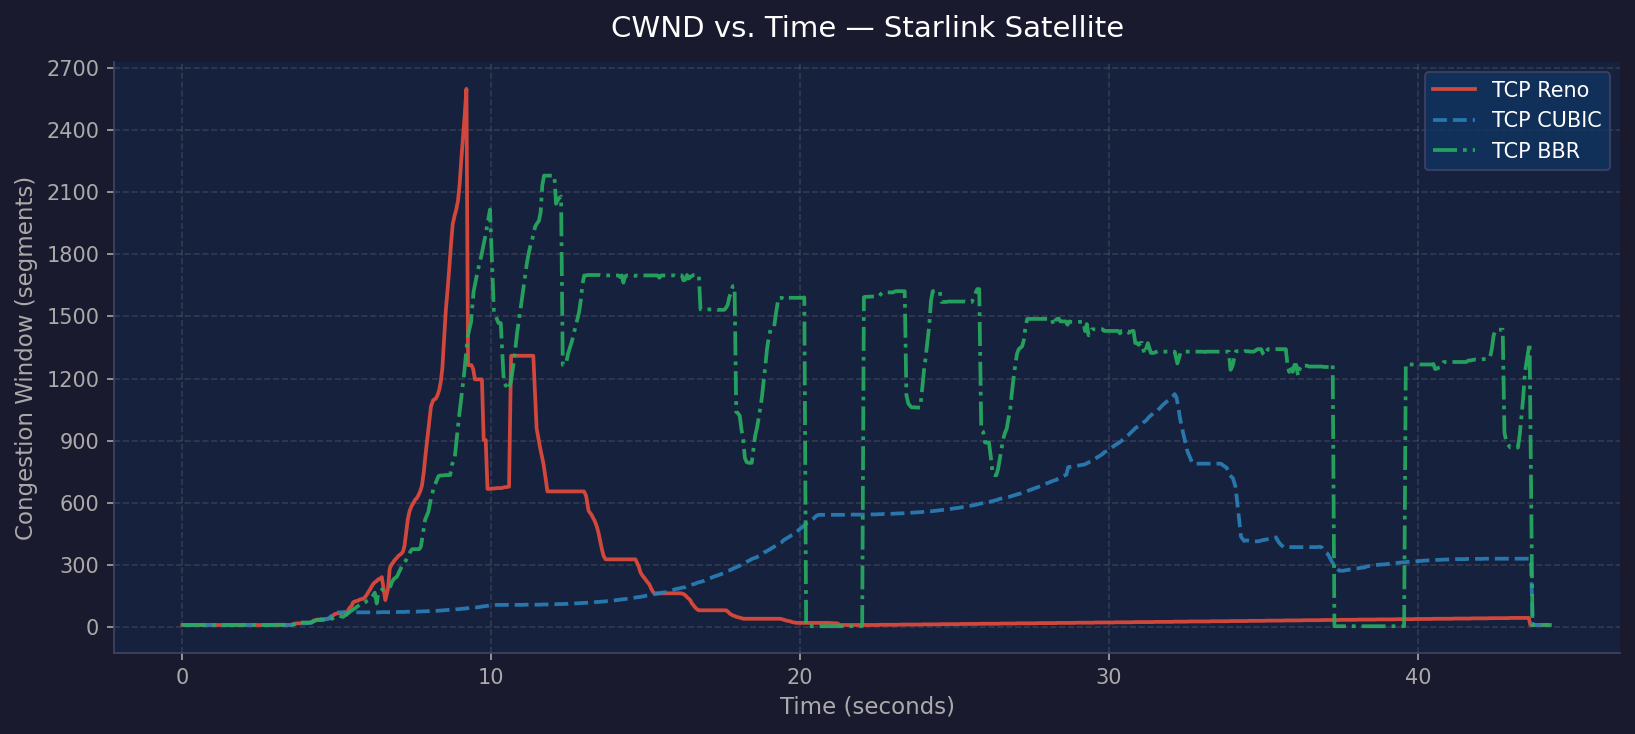
\includegraphics[width=\textwidth]{assets/plots/tcp_starlink_satellite_cwnd.png}
            \end{center}
        \end{column}
    \end{columns}
\end{frame}

% Section 5: Bufferbloat
\section{Scenario 3: Bufferbloat}
\begin{frame}{Scenario 3: The Bufferbloat Trap}
    \begin{columns}
        \begin{column}{0.5\textwidth}
            \begin{itemize}
                \item \textbf{Setup:} 10Mbps cap with a 50,000 packet queue.
                \item \textbf{CUBIC:} Meaningless scaling into the buffer; RTT grows to seconds.
                \item \textbf{BBR:} Locks at BDP, ignoring the bloated queue to preserve latency.
            \end{itemize}
        \end{column}
        \begin{column}{0.5\textwidth}
            \begin{center}
                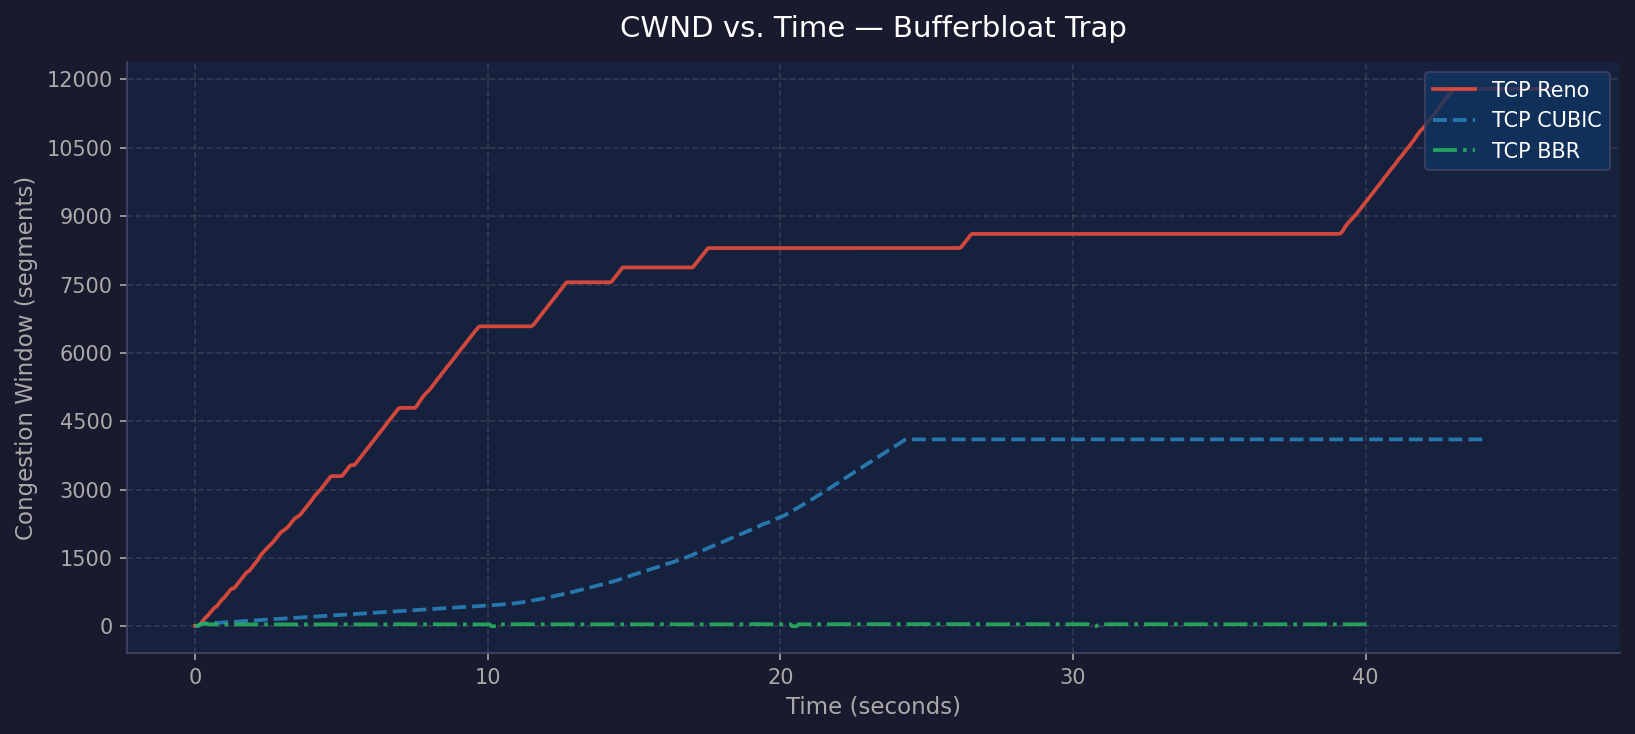
\includegraphics[width=\textwidth]{assets/plots/tcp_bufferbloat_cwnd.png}
            \end{center}
        \end{column}
    \end{columns}
\end{frame}

% Section 6: Summary
\begin{frame}{Comparative Summary}
    \begin{table}[]
        \begin{tabular}{l|c|c|r}
        \textbf{Algorithm} & \textbf{WiFi} & \textbf{Satellite} & \textbf{Bloat} \\ \hline
        TCP Reno           & Poor          & Failed             & Bloated        \\
        TCP CUBIC          & Fair          & Poor               & Bloated        \\
        TCP BBR            & \textbf{Excellent} & \textbf{Good} & \textbf{Target} \\
        QUIC               & TBD           & TBD                & TBD           
        \end{tabular}
    \end{table}
\end{frame}

\end{document}
